% This file was created by matlab2tikz.
%
%The latest updates can be retrieved from
%  http://www.mathworks.com/matlabcentral/fileexchange/22022-matlab2tikz-matlab2tikz
%where you can also make suggestions and rate matlab2tikz.
%
\definecolor{mycolor1}{rgb}{0.00000,0.44700,0.74100}%
\definecolor{mycolor2}{rgb}{0.85000,0.32500,0.09800}%
\definecolor{mycolor3}{rgb}{0.92900,0.69400,0.12500}%
\definecolor{mycolor4}{rgb}{0.49400,0.18400,0.55600}%
\definecolor{mycolor5}{rgb}{0.46600,0.67400,0.18800}%
\definecolor{mycolor6}{rgb}{0.30100,0.74500,0.93300}%
\definecolor{mycolor7}{rgb}{0.63500,0.07800,0.18400}%
%
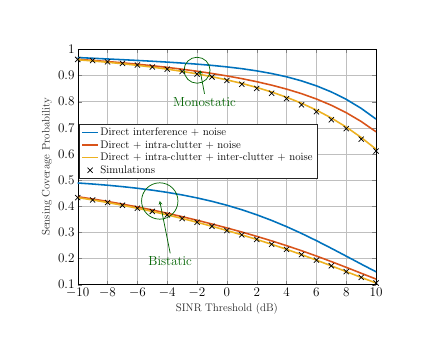
\begin{tikzpicture}[scale=0.33, transform shape,font=\Large]

\begin{axis}[%
width=4.521in,
height=3.566in,
at={(0.758in,0.481in)},
scale only axis,
xmin=-10,
xmax=10,
xlabel style={font=\large\color{white!15!black}},
xlabel={SINR Threshold (dB)},
ymin=0.1,
ymax=1,
ylabel style={font=\large\color{white!15!black}},
ylabel={Sensing Coverage Probability},
axis background/.style={fill=white},
xmajorgrids,
ymajorgrids,
legend style={at={(0.003,0.451)}, anchor=south west, legend cell align=left, align=left, draw=white!15!black,font=\large}
]
% \addplot [line width=0.6mm, color=mycolor1]
%   table[row sep=crcr]{%
% -10	0.9974\\
% -9	0.9967\\
% -8	0.9958\\
% -7	0.9947\\
% -6	0.9934\\
% -5	0.9916\\
% -4	0.9895\\
% -3	0.9868\\
% -2	0.9834\\
% -1	0.9792\\
% 0	0.9738\\
% 1	0.9672\\
% 2	0.9588\\
% 3	0.9485\\
% 4	0.9356\\
% 5	0.9196\\
% 6	0.8998\\
% 7	0.8755\\
% 8	0.8459\\
% 9	0.8101\\
% 10	0.7671\\
% };
% \addlegendentry{Noise effect only}

\addplot [line width=0.6mm, color=mycolor1]
  table[row sep=crcr]{%
-10	0.9685\\
-9	0.9659\\
-8	0.9631\\
-7	0.9604\\
-6	0.9575\\
-5	0.9544\\
-4	0.9511\\
-3	0.9474\\
-2	0.9433\\
-1	0.9385\\
0	0.9328\\
1	0.926\\
2	0.9176\\
3	0.9074\\
4	0.8949\\
5	0.8794\\
6	0.8604\\
7	0.8371\\
8	0.8087\\
9	0.7743\\
10	0.7331\\
};
\addlegendentry{Direct interference + noise}

\addplot [line width=0.6mm, color=mycolor2]
  table[row sep=crcr]{%
-10	0.9619\\
-9	0.9577\\
-8	0.9533\\
-7	0.9484\\
-6	0.9431\\
-5	0.9373\\
-4	0.9309\\
-3	0.9239\\
-2	0.9162\\
-1	0.9077\\
0	0.8983\\
1	0.8879\\
2	0.8762\\
3	0.863\\
4	0.8479\\
5	0.8305\\
6	0.8101\\
7	0.7861\\
8	0.7577\\
9	0.7241\\
10	0.6845\\
};
\addlegendentry{Direct + intra-clutter + noise}

\addplot [line width=0.6mm, color=mycolor3]
  table[row sep=crcr]{%
-10	0.9601\\
-9	0.9555\\
-8	0.9505\\
-7	0.9449\\
-6	0.9387\\
-5	0.9319\\
-4	0.9242\\
-3	0.9157\\
-2	0.9061\\
-1	0.8953\\
0	0.8832\\
1	0.8696\\
2	0.8542\\
3	0.8367\\
4	0.8167\\
5	0.7939\\
6	0.7676\\
7	0.7374\\
8	0.7027\\
9	0.663\\
10	0.6178\\
};
\addlegendentry{Direct + intra-clutter + inter-clutter + noise}




\addplot [color=white, draw=none, mark=x, thick, mark size=4pt, mark options={ black}]
  table[row sep=crcr]{%
-10	0.9613\\
-9	0.9569\\
-8	0.9521\\
-7	0.9461\\
-6	0.9399\\
-5	0.9323\\
-4	0.924\\
-3	0.915\\
-2	0.9052\\
-1	0.8942\\
0	0.8811\\
1	0.8664\\
2	0.8504\\
3	0.832\\
4	0.8114\\
5	0.7879\\
6	0.7613\\
7	0.7308\\
8	0.6968\\
9	0.6566\\
10	0.611\\
};
\addlegendentry{Simulations}






\addplot [line width=0.6mm, color=mycolor1]
  table[row sep=crcr]{%
-10	0.4889\\
-9	0.4849\\
-8	0.4803\\
-7	0.4749\\
-6	0.4687\\
-5	0.4614\\
-4	0.453\\
-3	0.4432\\
-2	0.4318\\
-1	0.4187\\
0	0.4037\\
1	0.3866\\
2	0.3673\\
3	0.3457\\
4	0.322\\
5	0.2961\\
6	0.2683\\
7	0.2391\\
8	0.2091\\
9	0.1788\\
10	0.1492\\
};


\addplot [line width=0.6mm, color=mycolor2]
  table[row sep=crcr]{%
-10	0.4364\\
-9	0.4277\\
-8	0.4183\\
-7	0.4081\\
-6	0.3972\\
-5	0.3856\\
-4	0.3732\\
-3	0.3601\\
-2	0.3464\\
-1	0.332\\
0	0.317\\
1	0.3013\\
2	0.2848\\
3	0.2675\\
4	0.2492\\
5	0.23\\
6	0.2096\\
7	0.1883\\
8	0.1663\\
9	0.1438\\
10	0.1214\\
};


\addplot [line width=0.6mm, color=mycolor3]
  table[row sep=crcr]{%
-10	0.433\\
-9	0.424\\
-8	0.4142\\
-7	0.4036\\
-6	0.3922\\
-5	0.38\\
-4	0.3669\\
-3	0.3531\\
-2	0.3386\\
-1	0.3233\\
0	0.3072\\
1	0.2905\\
2	0.2729\\
3	0.2545\\
4	0.2351\\
5	0.2149\\
6	0.1939\\
7	0.1721\\
8	0.15\\
9	0.1279\\
10	0.1064\\
};



\addplot [color=white, draw=none, mark=x, thick, mark size=4pt, mark options={ black}]
  table[row sep=crcr]{%
-10	0.433\\
-9	0.424\\
-8	0.4142\\
-7	0.4036\\
-6	0.3922\\
-5	0.38\\
-4	0.3669\\
-3	0.3531\\
-2	0.3386\\
-1	0.3233\\
0	0.3072\\
1	0.2905\\
2	0.2729\\
3	0.2545\\
4	0.2351\\
5	0.2149\\
6	0.1939\\
7	0.1721\\
8	0.15\\
9	0.1279\\
10	0.1064\\
};


\definecolor{darkgreen}{rgb}{0.00000,0.39200,0.00000} % Define dark green

\draw [stealth-,thick, darkgreen] (axis cs:-1.8,0.92) -- (axis cs:-1.5,0.83) node[below]{Monostatic};
\draw [thick, darkgreen] (-2,0.92) ellipse (0.5cm and 0.5cm); % Ellipse position unchanged

\draw [stealth-,thick, darkgreen] (axis cs:-4.5,0.42) -- (axis cs:-3.8,0.22) node[below]{Bistatic}; % Slightly lowered arrow
\draw [thick, darkgreen] (axis cs:-4.5,0.42) ellipse (0.7cm and 0.7cm); % Slightly lowered ellipse






\end{axis}



\begin{axis}[%
width=5.833in,
height=4.375in,
at={(0in,0in)},
scale only axis,
xmin=0,
xmax=1,
ymin=0,
ymax=1,
axis line style={draw=none},
ticks=none,
axis x line*=bottom,
axis y line*=left
]
\end{axis}
\end{tikzpicture}%